\section{Amélioration}


	Dans le but de simplifier l'expérience de l'utilisateur, nous avons souhaité ajouter certaines fonctionnalités à notre logiciel. Si celles-ci n'apportent pas d'amélioration en terme d'analyse des arbres, elles permettent de faciliter grandement leur modification. Nous distinguerons deux types de modifications : celles qui simplifient l'édition de l'arbre par l’intermédiaire d'AdTool, qui se traduiront par une modification de ce logiciel, et celles intégrées à \textbf{Glasir} qui simplifieront la navigation entre les différents arbres (qu'ils soient réalisés par l'utilisateur lui-même ou importés comme modèles). 

	\subsection{Liste d'arbres}.

	ADTool ne permet d'ouvrir qu'un seul arbre à la fois : cette limitation est particulièrement handicapante. Par exemple, l'utilisateur ne peut pas ouvrir deux versions différentes d'un même arbre pour les comparer. Notre logiciel rendra donc possible l'ouverture simultanée de plusieurs onglets, chacun possédant un arbre différent. 

	Cette fonctionnalité induit la possibilité pour l'utilisateur de manipuler un grand nombre d'arbres en simultané dans le cadre d'un même projet. Le module \emph{Liste d'arbres} fournira à l'utilisateur une présentation de la liste des arbres du projet sous forme d'arborescence. Il s'agira d'un dock disponible sur le côté du logiciel. 

	L'utilisateur aura aussi la possibilité de créer des catégories et des sous-catégories d'arbres pour hiérarchiser son projet. La suppression, la création et le renommage d'un arbre seront réalisables directement depuis ce module. 

	\subsection{Bibliothèque de modèles}


	La réalisation d'un arbre est un exercice de création. Il n'est pas toujours aisé de créer un arbre de but en blanc. Pour aider l'expert, \emph{Glasir} fournira à l'utilisateur une bibliothèque de modèle. Celle-ci contiendra un ensemble d'arbres génériques. L'utilisateur pourra utiliser ces arbres comme modèle pour créer un nouvel arbre ou directement l'utiliser en l'implémentant. La création d'un nouveau projet créer une copie de la bibliothèque de modèle qui devient modifiable pour l'utilisateur.		

	\subsection{Éditeur d'arbres}

	L'édition des arbres dans \emph{Glasir} se fera par l'intermédiaire d'ADtool. L'ouverture d'un arbre par l'utilisateur provoque le lancement d'une instance d'ADTool contenant cet arbre. Chaque instance d'ADTool étant imbriqué dans l'IHM de \emph{Glasir} sous la forme d'onglet. Dans le but de rendre possible l'interaction entre notre logiciel et ADtool, \emph{Glasir} fera tourner une version d'ADtool modifié. %moyen....

\subsection{Couper copier coller}
	
	ADTool ne permet pas l'utilisation du couper/copier-coller qui pourraient pourtant s'avérer précieuses lors de la création d'un arbre. Par exemple, dans le cas de l'oubli d'un nœud père, l'instauration de ces fonctionnalités permettra de déplacer facilement les fils concernés de l'ancien au nouveau nœud père.
	En conséquence, la sélection d'un nœud entraînera la sélection de ses fils, afin de pouvoir effectuer des transferts rapidement. Ceci sera automatique, car nous avons considéré que la sélection partielle des nœuds fils n'apportait pas d'amélioration utile. Le système de raccourcis clavier classique ne sera probablement pas repris, au profit d'une gestion à la souris, et d'un affichage spécial des nœuds copiés.

	Cependant, cette fonction entraîne une nécessité de cohérence. En effet, des nœuds de même nom ne pourront pas être présents, il faudra donc gérer ces cas de figure. L'édition XML abordée ci-dessous sera le plus simple dans ce cas.
	%- Sélection d'un noeud (ça sélectionne aussi ses fils) : repérée par une coloration du noeud sélectionné
	%- Clic droit sur le noeud sélectionné pour le copier/couper ainsi que ses fils
	%- Pour coller on clique droit sur un noeud et cela rajoute l'arbre copié en tant que nouveau fils
	%- On peut le faire entre différentes instances d'ADTool
	%- Sanity check : faire attention au nom des labels

	\subsection{Amélioration du codage des arbres}

	Dans sa version actuelle, ADTool affiche dans son interface un section nommée \emph{ADTerm Edit}. Celle-ci affiche une représentation de l'arbre sous la forme d'un texte utilisant un langage propre au logiciel. Lors de la modification de l'arbre dans l'éditeur graphique, AdTool modifie le code en temps réel. On peut ainsi modifier facilement les labels des nœuds présents, ou changer un opérateur directement depuis \emph{ADTerm Edit} puis valider afin d'afficher le résultat sous forme d'arbre. 

	Mais le langage qui permet de décrire les arbres ne contient pas le nom des autres nœuds que les feuilles. Sur la figure \ref{fig:int_adTool}, on peut constater que le code indique le nom des deux feuilles \textit{Acheter le matériel nécessaire} et \textit{Essayer les clés de chiffrage}, que la conjonction est bien précisé par l'opérateur \textit{ap} mais qu'aucune référence n'est faite au label du nœud parent (\textit{Casser le chiffrage}).

	Pour remédier à ce problème, nous créerons une nouvelle grammaire corrigeant ce défaut.

	%- Ajouter la possibilité d'éditer l'arbre directement en xml. Possibilité de masquer/afficher le bloc xml.
	%- Ajouter nœud père dans l'éditeur texte 


	% ATTENTION  !! CHANGER CRIPTAGE EN CHIFFFRAGE !!!
	\begin{figure}
		\centering
		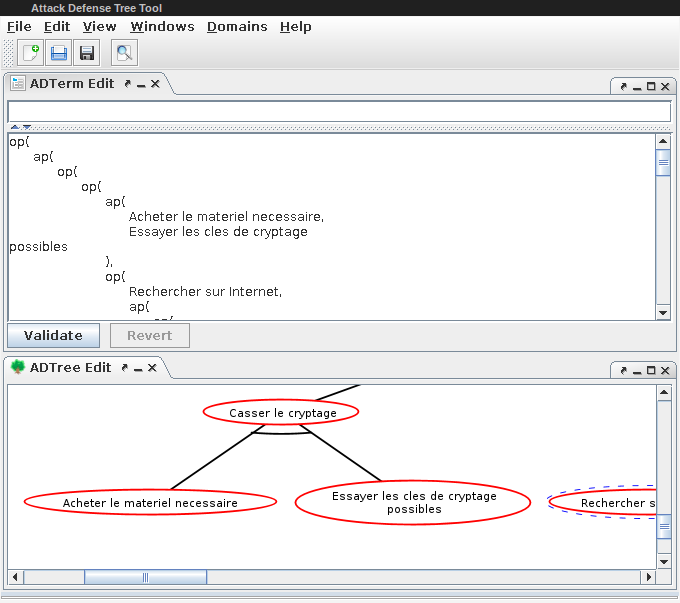
\includegraphics[width=0.5\textwidth]{figure/interface_adtool.png}
		\caption{L'interface d'AdTool.}
		\label{fig:int_adTool}
	\end{figure}
	
	\subsection{CTRL-Z}
	Pour le moment, effectuer une action est irréversible. Un renommage ou l'ajout d'une feuille est rapide à effectuer, mais supprimer par erreur un nœud peut entraîner un travail énorme. La possibilité de faire un retour à l'état précédent de l'arbre éviterait d'avoir à recommencer ce travail de construction fastidieux. Nous souhaitons créer au moins une sauvegarde de l'état précédent, afin de pouvoir annuler la dernière modification. Si possible, l'implémentation d'une pile circulaire contenant les N derniers états avec un curseur pointant sur l'état courant, permettra de revenir en arrière sans contraintes.
	%- Annulation d'une ou plusieurs des modifications précédentes
	%- Coder une pile d'états avec un curseur qui indique l'état courant
	%- Chaque action entraîne la création d'un nouvel état
	
	\subsection{Paramètre de synthèse}
	Comme précisé plus haut, ADTool met à notre disposition treize paramètres de base afin de donner des valuations à l'arbre. Afin de rendre complète l'éditeur de paramètres que nous souhaitons implémenter, nous serons amenés à ajouter des paramètres de base, permettant de créer des fonctions complètes. Des paramètres tels que le coût financier, humain ou le temps nécessaire à la réalisation sont souvent ressortis dans nos exemples d'attaque du réseau STAR. Ceux-ci pourront se combiner afin de réaliser des fonctions dont aurait besoin un expert en sécurité désirant réaliser l'analyse d'un système.
	%- ajouter un paramètre de plus de disponible dans AdTool pour les fonctions de synthèse.
		
	\subsection{Vue globale des paramètres}
	Dans l'état actuel d'ADTool, un seul paramètre est affiché, même si plusieurs paramètres servent à valuer le nœud. En effet, les paramètres ont un onglet propre, et un seul est effectivement affiché. Nous souhaitons créer un onglet général, regroupant tous les paramètres appliqués, afin d'avoir une vision plus globale de l'avancée de notre travail, et ainsi faciliter la création des fonctions de synthèse.
	Pour une meilleure lisibilité, les différents paramètres auront chacun une couleur différente, accompagnée d'une légende résumant à quoi elles correspondent.
	Nous devrons également gérer la taille des nœuds, pour que les paramètres ne dépassent pas de la bulle. Un tel système est déjà présent dans ADTool afin de gérer les labels, il suffira de l'étendre à l'affichage des paramètres.
 	%Pour le moment, un onglet dans ADTool par paramètre (sur l'arbre, seul ce paramètre est apparent)	
	%- Créer un nouvel onglet plus global avec tous les paramètres visibles sous les labels, chaque paramètre d'une couleur différente (légende %explicative sur le coté)
	%- Attention à ce que les paramètres ne débordent pas des nœuds, il faut éventuellement élargir les ronds
